%Noise Generator Module

\subsubsection{Overview}
\label{Noise Generator}
\index{Noise Generator}\index{utilities, Noise Generator}

\begin{figure}[h]
\begin{center}
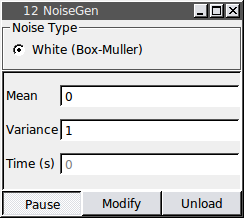
\includegraphics[width=2in]{noisegen.png} 
\caption[Noise Generator]{The noise generator module outputs Gaussian white noise.} 
\end{center}
\label{wavemaker}
\end{figure}

The noise generator module can continuously generate Gaussian white noise computed using the Box-Muller method.

\subsubsection{Output Channels}
\begin{description}
\item [Noise Waveform]Noise output
\end{description}

\subsubsection{Parameters}
\begin{description}
\item [Mean]Mean value of noise output
\item [Variance]The given variance used in noise calculated
\end{description}